\documentclass[tikz]{standalone}
\usepackage{amsmath}
\begin{document}
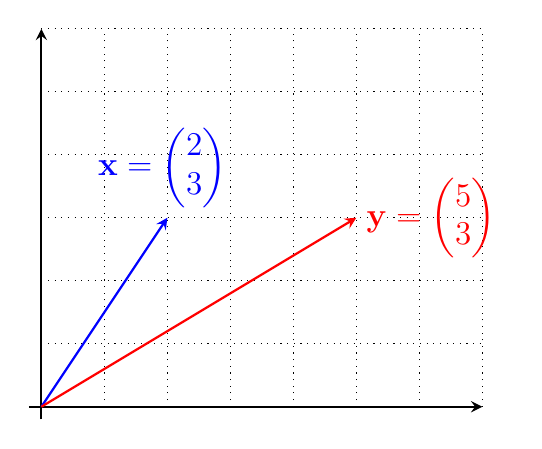
\begin{tikzpicture}[scale=0.8]

% axes
  \draw[thick,>=stealth,->]           (0,-0.2) -- (0,6);
  \draw[thick,>=stealth,->]           (-0.2,0) -- (7,0);

% grid lines
    \draw[step=1.0,black,thin,dotted,xshift=1cm,yshift=1cm] (-1,-1) grid (6,5);

% starting vector blue, transformed vector red
  \draw[thick,>=stealth,->,draw=blue] (0,0) -- (2,3)  node[above, text=blue, text width=5em] (x) {\large $\mathbf{x=\begin{pmatrix}2 \\ 3 \end{pmatrix}}$};
  \draw[thick,>=stealth,->,draw=red ] (0,0) -- (5,3)  node[right, text=red,  text width=5em] (y) {\large $\mathbf{y=\begin{pmatrix}5 \\ 3 \end{pmatrix}}$};

\end{tikzpicture}
\end{document}